\documentclass[10pt]{beamer}

\usetheme[progressbar=head]{moloch}

\usepackage[utf8]{inputenc}

% Essential packages
\usepackage{listings}
\usepackage{mathtools}
\usepackage{tikz}
\usepackage{svg}
\usepackage{booktabs}
\usepackage{ccicons}
\usepackage{pgfplots}
\usepgfplotslibrary{dateplot}
\usepackage{xspace}
\usepackage[dvipsnames]{xcolor}
\usepackage{hyperref}

\hypersetup{
    colorlinks=true,
    linkcolor=blue,
    filecolor=magenta,      
    urlcolor=cyan,
    pdftitle={Overleaf Example},
    pdfpagemode=FullScreen,
    }

% Configure Moloch theme settings
\molochset{
    sectionpage=none,
    block=fill
}

\usefonttheme{professionalfonts}
\usepackage{bm}

% Progress bar

\setbeamertemplate{page number in head/foot}[totalframenumber]

\makeatletter
\setlength{\moloch@progressinheadfoot@linewidth}{1em}

\addtobeamertemplate{headline}{% 
    \begin{beamercolorbox}[colsep=1.5pt]{upper separation line head}
    \end{beamercolorbox}
    \begin{beamercolorbox}{section in head/foot}
        \vskip2pt\insertnavigation{\paperwidth}\vskip2pt
    \end{beamercolorbox}%
    \begin{beamercolorbox}[colsep=1.5pt]{lower separation line head}
    \end{beamercolorbox}
    \par
}{}

\setbeamertemplate{footline}{
    \begin{tikzpicture}[remember picture,overlay]
      \node[anchor=north east] at ([yshift=-5.5ex]current page.north east) {\usebeamercolor[fg]{page number in head/foot}\usebeamertemplate{page number in head/foot}};
    \end{tikzpicture}
}

\def\beamer@writeslidentry{\clearpage\beamer@notesactions}  
\makeatother

\setbeamercolor{section in head/foot}{fg=black, bg=white}

\setbeamercolor{page number in head/foot}{fg=mLightBrown}



% Encoding and localization
\usepackage[utf8]{inputenc}
\usepackage[T2A]{fontenc}
\usepackage[english]{babel}

% Code listing settings
\definecolor{mauve}{rgb}{0.58,0,0.82}
\definecolor{dkgreen}{rgb}{0,0.4,0}
\definecolor{gray}{rgb}{0.5,0.5,0.5}
\definecolor{lightgray}{rgb}{0.95,0.95,0.95}

\lstset{
  language=Python,
  basicstyle=\fontsize{5}{6}\ttfamily,
  numbers=left,
  stepnumber=1,
  numbersep=0.7em,
  backgroundcolor=\color{lightgray},
  showspaces=false,
  showstringspaces=false,
  showtabs=false,
  frame=single,
  rulecolor=\color{black},
  tabsize=2,
  breaklines=true,
  breakatwhitespace=false,
  identifierstyle=\color{blue!25!black},  
  keywordstyle=\color{blue!90!black},
  commentstyle=\color{dkgreen},
  stringstyle=\color{mauve},
  escapeinside={\`}{\`}, 
  escapebegin=\color{gray!50!black}\footnotesize,
  keepspaces=true,
  columns=fullflexible
}

% Presentation title and metadata
\title{W0: Vectors and linear combinations}
\date{19.09.2025}
\author{Oleksandr Kulkov}
\institute{ETH Zürich}
\titlegraphic{\hfill\includesvg[height=0.5cm]{../img/svg/eth}}


\begin{document}

\maketitle

\section{Intro}
\begin{frame}{Group info}
    \textbf{Group}: 24

    \textbf{Location}: CHN G 46
    
    \textbf{Teaching assistant}: Oleksandr Kulkov

    \textbf{Language}: English

    \textbf{Focus group}\footnote{More thorough and detailed explanation of basics}: Yes

    \textbf{Website}: \small\url{https://ti.inf.ethz.ch/ew/courses/LA25}

    Please don't hesitate to interrupt at any moment if have any questions!
\end{frame}

\begin{frame}{Introductions}
    Let's get to know each other!

\begin{block}{Intro questions}
    \begin{itemize}
        \item Your name?
        \item A bit about yourself?
        \item What do you expect from a focus group?
    \end{itemize}
\end{block}
\end{frame}

\begin{frame}{Course info}
\begin{itemize}
    \item Exam structure:
    \begin{itemize}
        \item \textbf{Calculations}: Solve standard compute tasks (answer-only);
        \item \textbf{Proofs}: Need to justify anything that wasn't in \textit{lectures};
        \item \textbf{Multi-choice questions}: Pick the only correct option;
    \end{itemize}
    \item Weekly bonus tasks: up to 0.25 extra points to grade;
    \item Hand-ins: One exercise per week, get feedback;
\end{itemize}
\end{frame}

\section{Scalars}
\begin{frame}{Scalars}
    Recall ``standard'' sets of numbers:

    \begin{itemize}
        \item $\mathbb N$: \textbf{Natural} numbers;
        \item $\mathbb Z$: \textbf{Integer} numbers;
        \item $\mathbb Q$: \textbf{Rational} numbers;
        \item $\mathbb R$: \textbf{Real} numbers;
    \end{itemize}

    Represent \textit{quantity}, typically called the \textbf{scalars}\footnote{from ``scale''}.
\end{frame}

\section{Tuples}
\begin{frame}{Tuples}
    $\mathbb R^m$ is the set of \textbf{tuples}: $\mathbb R^m = \{(x_1,\dots,x_m) : x_i \in \mathbb R\}$\footnote{$x_i \in \mathbb R$ means that $x_i$ is an \textit{element} of the \textit{set} $\mathbb R$}:

    \begin{itemize}
        \item $\mathbb R^2 = \{(x, y) : x, y \in \mathbb R\}$ -- points of a 2D \textbf{plane};
        \item $\mathbb R^3 = \{(x, y, z): x, y, z \in \mathbb R\}$ -- points of a 3D \textbf{space};
    \end{itemize}

    The \textbf{power} symbol corresponds to the \textbf{Cartesian product}:
    $$
    A \times B = \{(a, b) : a \in A \text{ and } b \in B\}
    $$
    We may use \textit{indices} to refer to the \textit{components} of a tuple.
\end{frame}

\section{Vectors}
\begin{frame}{Vectors}
    \textbf{Real vectors}\footnote{in our course, denoted by lowercase \textbf{bold} letters} are elements of a set $V$, called \textbf{vector space}, with:

    \begin{itemize}
        \item \textbf{Addition}: $\mathbf{u} + \mathbf{v} \in V$ for $\mathbf{u}, \mathbf{v} \in V$;
        \item \textbf{Scaling}: $k \mathbf{v} \in V$ for $k \in \mathbb R$ and $\mathbf{v} \in V$;
    \end{itemize}

    Addition and scaling are collectively called \textbf{linear operations}\footnote{hence, they are the subject of \textit{linear} algebra}.

    In most general case, addition and scaling are \textbf{axiomatic}\footnote{defined by their properties}.

    In our course, we will mostly work with $V = \mathbb R^m$.
\end{frame}

\begin{frame}{Column vectors}
    For $V = \mathbb R^m$, our course uses columns to represent vectors:
    $$
    \mathbf v = \begin{bmatrix}
        v_1 \\ v_2 \\ \vdots \\ v_m
    \end{bmatrix},
    $$
    and the addition and scaling are \textbf{component-wise}:
    \begin{itemize}
        \item $(\mathbf u + \mathbf v)_i = u_i + v_i$;
        \item $(k \mathbf v)_i = k v_i$;
    \end{itemize}

    This is geometry-motivated for $m=2$ and $m=3$.
\end{frame}

\begin{frame}{Core properties}
    \begin{block}{Vector addition properties\footnote{in abstract algebra sense, vector space is a commutative group}}
    \begin{itemize}
        \item Associativity: $\mathbf u + (\mathbf v + \mathbf w) = (\mathbf u + \mathbf v) + \mathbf w$;
        \item Commutativity: $\mathbf u + \mathbf v = \mathbf v + \mathbf u$;
        \item Zero vector: $\mathbf v + \mathbf 0 = \mathbf 0 + \mathbf v = \mathbf v$;
        \item Negatives: $\mathbf v + (-\mathbf v) = \mathbf 0$;
    \end{itemize}
    \end{block}
    \begin{block}{Scaling properties}
        \begin{itemize}
            \item Compatibility with multiplication of scalars: $\alpha (\beta \mathbf v) = (\alpha \beta) \mathbf v$;
            \item Unit scaling: $1 \mathbf v = \mathbf v$;
            \item Distributivity with vector addition: $\alpha (\mathbf u + \mathbf v) = \alpha \mathbf u + \alpha \mathbf v$;
            \item Distributivity with scalar addition: $(\alpha+\beta) \mathbf v = \alpha \mathbf v + \beta \mathbf v$;
        \end{itemize}
    \end{block}
\end{frame}

\section{Geometry}
\begin{frame}{Vector geometry}
    In geometry, vectors have \textit{direction} and \textit{magnitude}\footnote{but \textbf{not} origin!}:

    \begin{center}
        \includesvg[height=4cm]{../img/svg/Vector_addition2}
        \includesvg[height=4cm]{../img/svg/Scalar_multiplication_of_vectors}
        
        {\small{\textit{Addition adds vector direction, scaling changes magnitude}}}
    \end{center}
\end{frame}

\begin{frame}{Linear combinations}

    A \textbf{linear combination} of $\mathbf v_1, \dots, \mathbf v_n \in V$ with coeffs. $\alpha_1,\dots,\alpha_n \in \mathbb R$:
    $$
    \alpha_1 \mathbf{v}_1 + \dots+\alpha_n \mathbf{v}_n \in V
    $$
    Some $\alpha_i$ may be zero. \textbf{Trivial} combination: $\alpha_1=\dots=\alpha_n = 0$.

\end{frame}

\begin{frame}{Special combinations}
    \begin{center}
        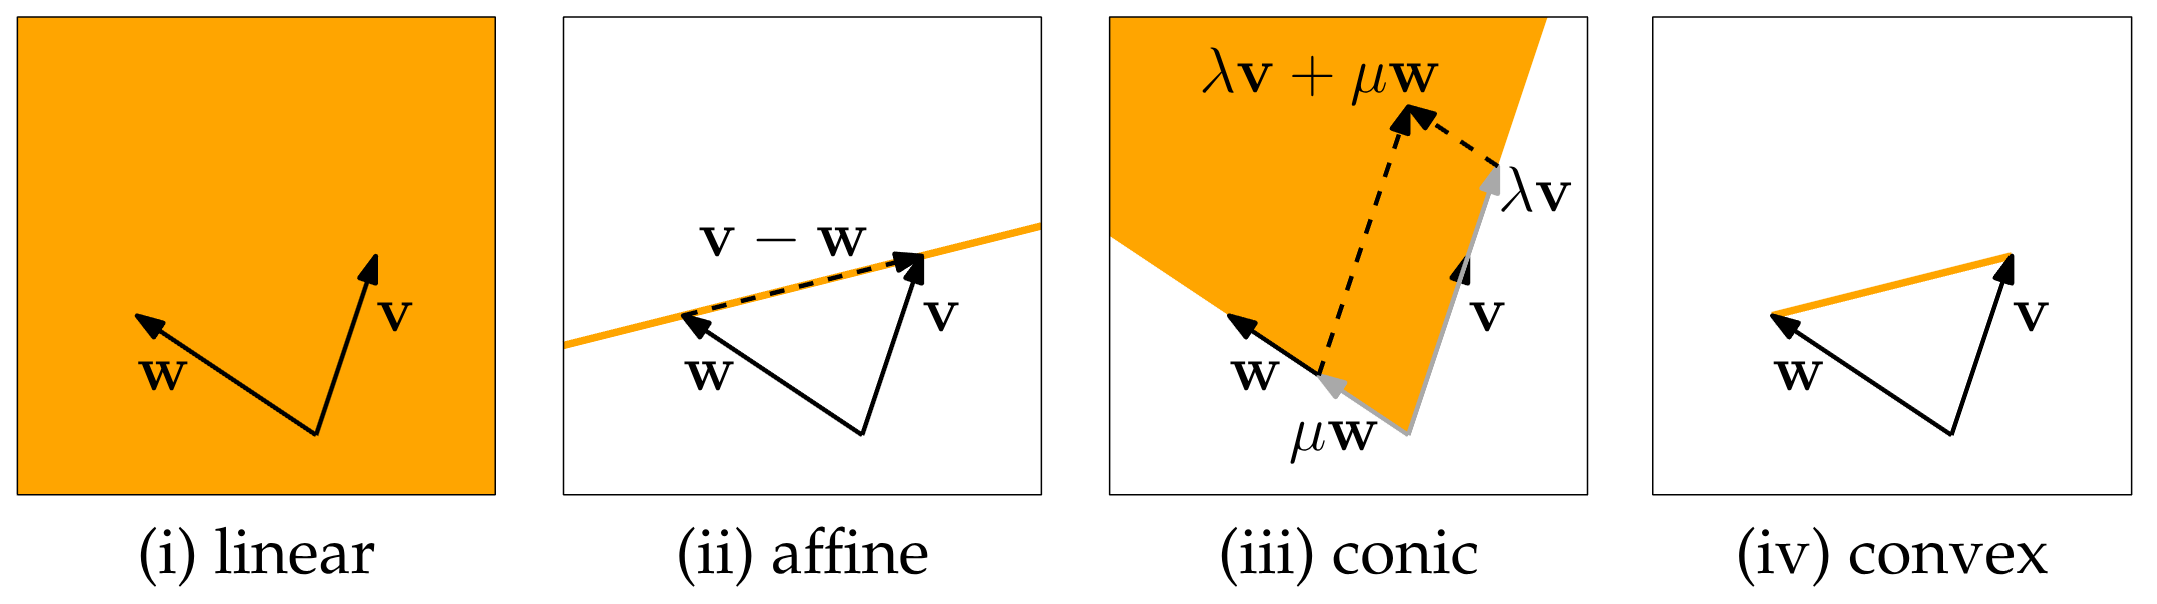
\includegraphics[height=3cm]{../img/png/combinations}
    \end{center}

    \begin{itemize}
        \item Affine: $\alpha_1 + \dots + \alpha_n = 1$;
        \item Conic: $\alpha_1, \dots, \alpha_n \geq 0$;
        \item Convex: $\alpha_1 + \dots + \alpha_n = 1$ \textit{and} $\alpha_1, \dots, \alpha_n \geq 0$.
    \end{itemize}
    
    We can rewrite $\alpha_1+\dots+\alpha_n=1$ as $\alpha_1 = 1-\alpha_2-\dots-\alpha_n$:
    $$
    \mathbf v_1 + \alpha_2 (\mathbf v_2 - \mathbf v_1) + \dots + \alpha_n(\mathbf v_n - \mathbf v_1) \in V
    $$

    Thus, affine combinations are linear combinations with ``shifted'' origin.
\end{frame}

\section{Exercises}
\begin{frame}{Triangle combinations}
    \begin{block}{Statement}
        Sketch sets of all possible linear, affine, conic and convex combinations of $3$ distinct points on a plane. Consider all cases.
    \end{block}
\end{frame}

\begin{frame}{Triangle combinations}
    Linear: The whole plane or a line (if collinear with $0$).

    Affine: The whole plane or a line (if collinear).

    Conic: The area between ``tangent'' rays or the whole plane (if $0$ is inside).

    Convex: The triangle spanned on the $3$ points.
\end{frame}

\begin{frame}{The perfect long drink (a)}
    \begin{block}{Statement}
    You have drinks $G$ and $T$. You have two drinks:
    \begin{enumerate}
        \item $15$ ml of $G$ and $85$ ml of $T$;
        \item $35$ ml of $G$ and $65$ ml of $T$;
    \end{enumerate}

    Can we mix a perfect drink ($23$ ml of $G$ and $77$ ml of $T$)?
    \end{block}
\end{frame}

\begin{frame}{The perfect long drink (a)}
    Use $x$ of first drink and $y$ of second drink:
    $$
    x \begin{bmatrix}15 \\ 85\end{bmatrix} + y \begin{bmatrix}35 \\ 65\end{bmatrix} = \begin{bmatrix}23 \\ 77\end{bmatrix} \iff \begin{cases}
        15x + 35y = 23 \\
        85x + 65y = 77
    \end{cases}
    $$
    Add equations: $$100(x+y) = 100 \iff x + y = 1$$

    Substitute $x=1-y$ into first equation:
    $$
    15(1-y) + 35y = 23 \iff 20y = 8 \iff y = \frac{2}{5}
    $$
    From $x=1-y$, we get $x = \frac{3}{5}$. It's feasible, because $0 \leq x, y \leq 1$.
\end{frame}

\begin{frame}{The perfect long drink (b)}
    \begin{block}{Statement}
        Consider the set of all $100$ ml drinks:
        $$
        D = \left\{\begin{bmatrix}g \\ t\end{bmatrix} \in \mathbb R^2 : g, t \geq 0 \text{ and }g+t=100\right\}
        $$
        For $\mathbf{v} = \begin{bmatrix}15 \\ 85\end{bmatrix}$ and $\mathbf{w} = \begin{bmatrix}35\\65\end{bmatrix}$, which $100$ ml drinks can be mixed?
    \end{block}
\end{frame}

\begin{frame}{The perfect long drink (b)}
    Any mix can be represented as $x \mathbf{v} + y \mathbf{w}$, where $x, y \geq 0$.

    Since initial drinks are $100$ ml, final drink volume is $x \cdot 100 + y \cdot 100$.

    We need it to still be $100$, hence $(x + y) \cdot 100 = 100 \iff x+y=1$.

    On the other hand, it is also sufficient for the drink to be in $D$, thus
    $$
    \hat D = \{x\mathbf v + y \mathbf w : x, y \geq 0 \text{ and } x+y=1\}
    $$
    $\hat D$ are convex combinations of $\mathbf v$ and $\mathbf w$, aka the segment between them.
\end{frame}

\begin{frame}{The perfect long drink (c)}
    \begin{block}{Statement}
        For $\mathbf{v} = \begin{bmatrix}15 \\ 85\end{bmatrix}$ and $\mathbf{w} = \begin{bmatrix}35\\65\end{bmatrix}$, which (any) drinks can be mixed?
    \end{block}
\end{frame}

\begin{frame}{The perfect long drink (c)}

    \begin{center}
        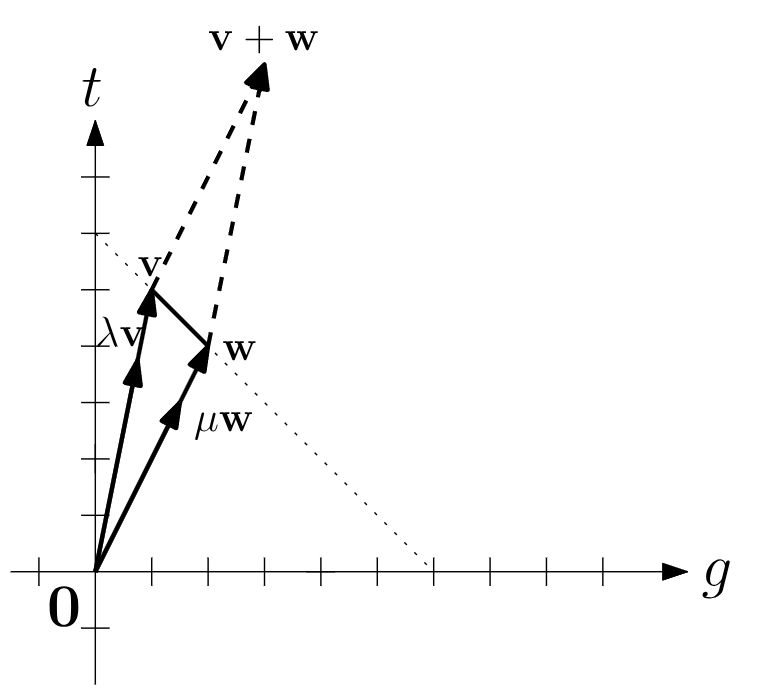
\includegraphics[height=4cm]{../img/png/2.c}
    \end{center}

    Since the drink no longer needs to be $100$ ml, we get rid of $x+y=1$.

    But, it should be $x, y \leq 1$, as we can't use more than $100\%$ of a drink.
    $$
    \bar D = \{x \mathbf v + y \mathbf w : 0 \leq x, y \leq 1\}
    $$
    $\bar D$ is a parallelogram spanned on $\mathbf 0$, $\mathbf v$, $\mathbf w$ and $\mathbf v + \mathbf w$.
\end{frame}

\begin{frame}{Geometry of linear combinations (a)}
    \begin{block}{Statement}
        Sketch the following set in $\mathbb R^3$:
        $$\left\{\lambda_1 \begin{bmatrix}-1 \\ 1 \\ 1\end{bmatrix} + \lambda_2 \begin{bmatrix}-2 \\ 2 \\ 2\end{bmatrix} + \lambda_3 \begin{bmatrix}-3 \\ 3 \\ 3\end{bmatrix} : \lambda_1, \lambda_2, \lambda_3 \in \mathbb R\right\}$$
    \end{block}
\end{frame}

\begin{frame}{Geometry of linear combinations (a)}

    \begin{center}
        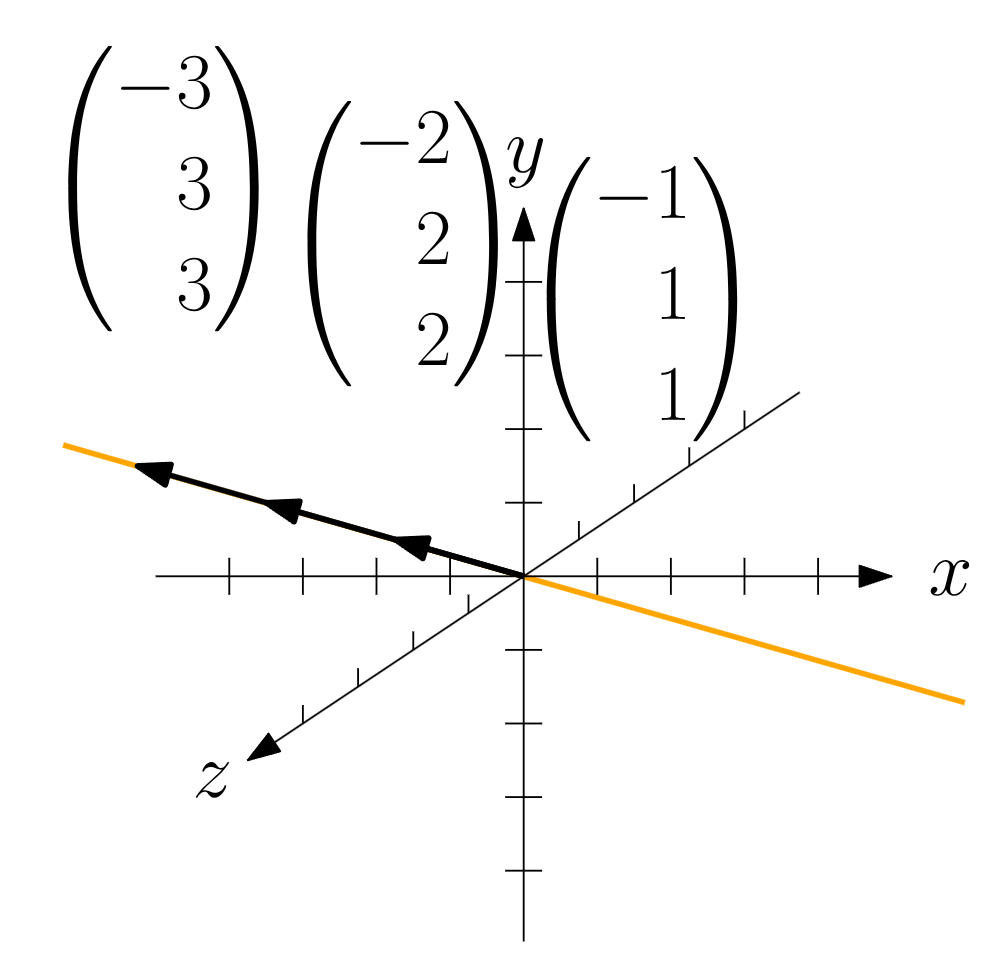
\includegraphics[height=5cm]{../img/png/3.a}
    \end{center}

    lets use $\mathbf a$, $\mathbf b$ and $\mathbf c$ to denote vectors. Note that $\mathbf b = 2 \mathbf a$ and $\mathbf c = 3 \mathbf a$.

    We can safely remove vectors that are linear combinations of others.

    Thus, the set is simply $\lambda_1 \mathbf a$, aka the line going through $\mathbf 0$ and $\mathbf a$.
\end{frame}

\begin{frame}{Geometry of linear combinations (b)}
    \begin{block}{Statement}
        Sketch the following set in $\mathbb R^3$:
        $$\left\{\lambda_1 \begin{bmatrix}-1 \\ 1 \\ 3\end{bmatrix} + \lambda_2 \begin{bmatrix}-2 \\ 2 \\ 0\end{bmatrix} + \lambda_3 \begin{bmatrix}-3 \\ 3 \\ 3\end{bmatrix} : \lambda_1, \lambda_2, \lambda_3 \in \mathbb R\right\}$$
    \end{block}
\end{frame}

\begin{frame}{Geometry of linear combinations (b)}

    \begin{center}
        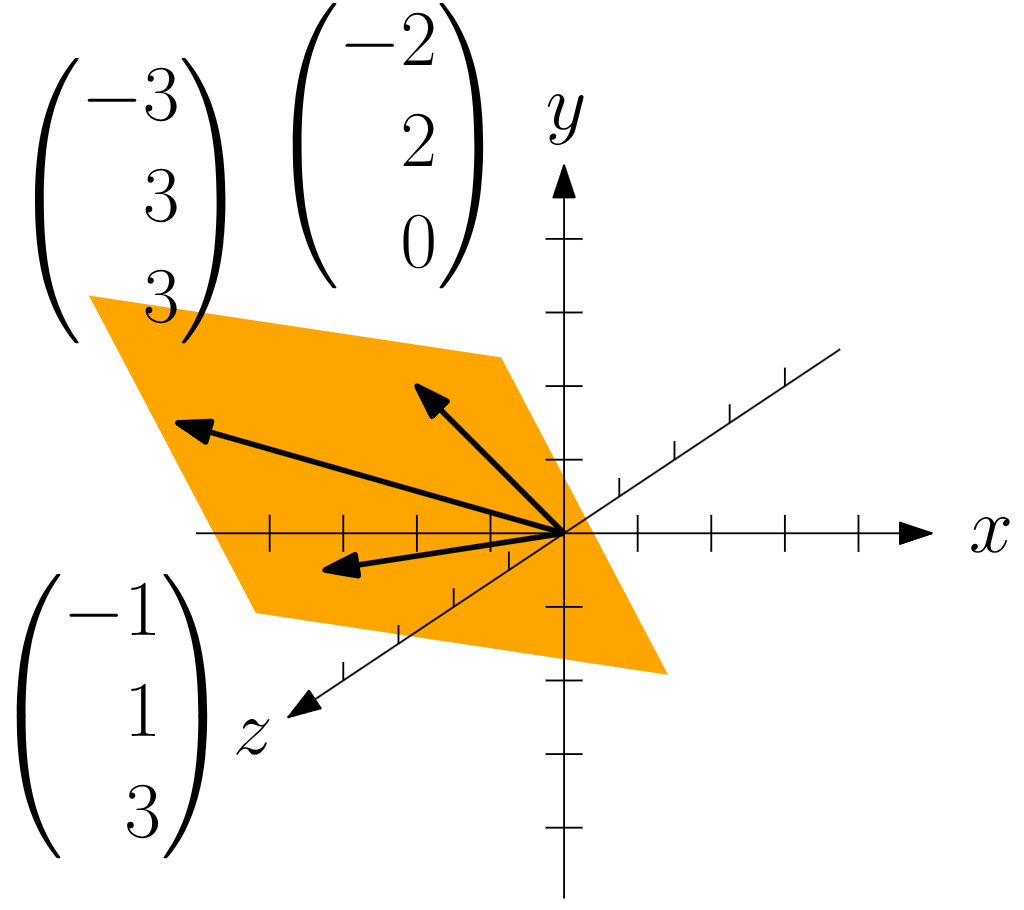
\includegraphics[height=5cm]{../img/png/3.b}
    \end{center}

    Note that $\mathbf c = \mathbf a + \mathbf b$, so we can ``ignore'' $\mathbf c$.

    Thus, the set is $\lambda_1 \mathbf a + \lambda_2 \mathbf b$, a plane passing through $\mathbf 0$, $\mathbf a$ and $\mathbf b$.
\end{frame}

\begin{frame}{Geometry of linear combinations (c)}
    \begin{block}{Statement}
    Sketch the following set in $\mathbb R^3$:
    $$\left\{\lambda_1 \begin{bmatrix}-1 \\ 1 \\ 3\end{bmatrix} + \lambda_2 \begin{bmatrix}-2 \\ 2 \\ 0\end{bmatrix} + \lambda_3 \begin{bmatrix}2 \\ 3 \\ -1\end{bmatrix} : \lambda_1, \lambda_2, \lambda_3 \in \mathbb R\right\}$$
    \end{block}
\end{frame}

\begin{frame}{Geometry of linear combinations (c)}
    \begin{center}
        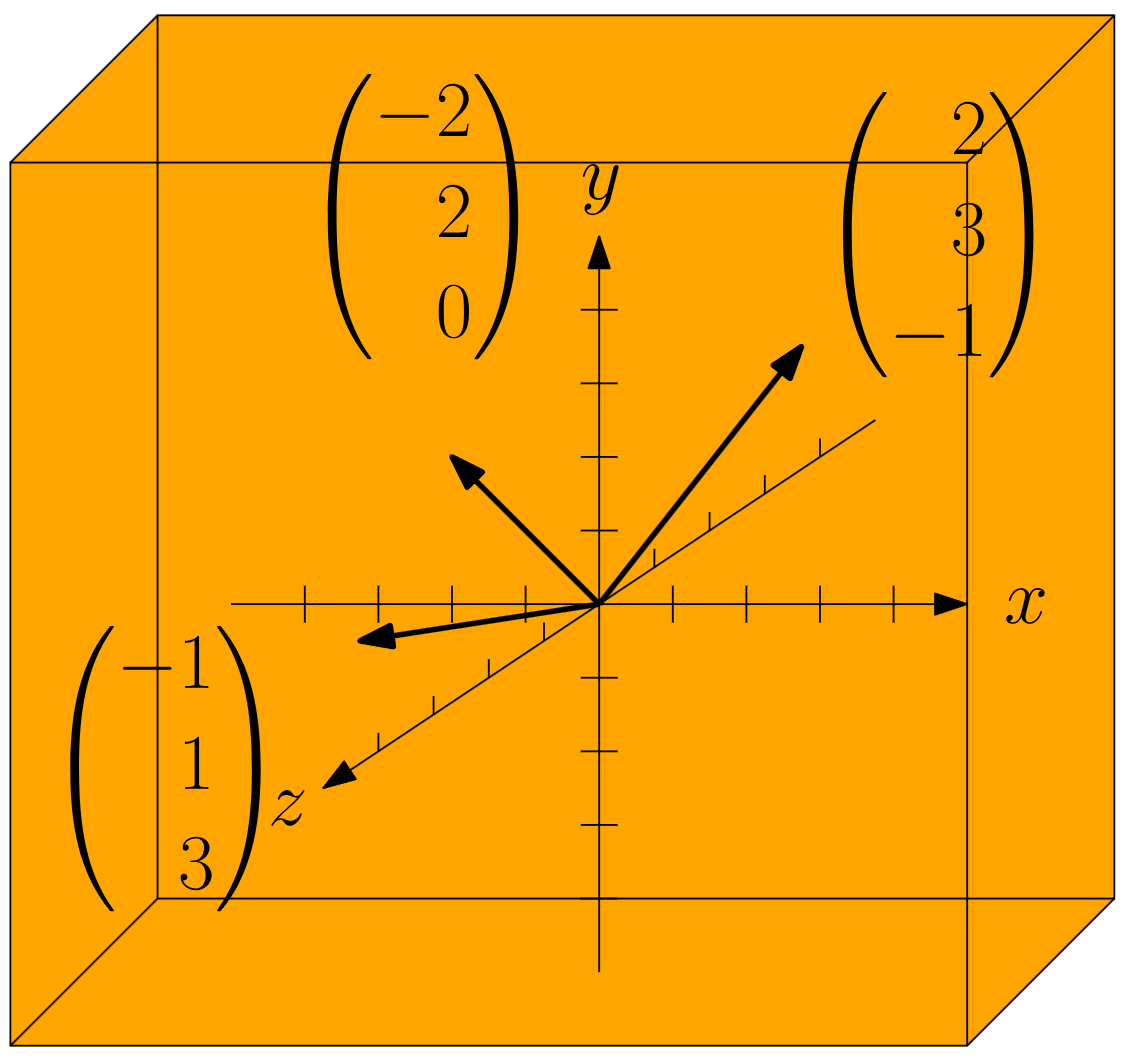
\includegraphics[height=5cm]{../img/png/3.c}
    \end{center}

    Vectors point in three independent directions.

    The set of all linear combinations covers the whole $\mathbb R^3$.
\end{frame}

\end{document}